\documentclass[11pt,letterpaper]{article}
\usepackage[top=1in,bottom=1in,left=1in,right=1in]{geometry}
\usepackage[numbers]{natbib}      % http://merkel.zoneo.net/Latex/natbib.php
\usepackage{lmodern}
\renewcommand\familydefault{\sfdefault} 
\usepackage[T1]{fontenc}

\bibpunct{(}{)}{;}{a}{,}{,}
\usepackage{chngpage}
\usepackage{stmaryrd}
\usepackage{amssymb}
\usepackage{amsmath}
\usepackage{amsthm}
\usepackage{graphicx}
\usepackage{lscape}
\usepackage{subfigure}
\usepackage{parskip}
\usepackage{algpseudocode}
\usepackage{algorithm}
\usepackage[usenames,dvipsnames]{color}
\usepackage{indentfirst}
\definecolor{myblue}{rgb}{0,0.1,0.6}
\definecolor{mygreen}{rgb}{0,0.3,0.1}
\usepackage[colorlinks=true,linkcolor=black,citecolor=mygreen,urlcolor=myblue]{hyperref}
\newcommand{\bocomment}[1]{\textcolor{Bittersweet}{[#1 -BTO]}}
\newenvironment{itemizesquish}{\begin{list}{\labelitemi}{\setlength{\parskip}{0.6cm}\setlength{\itemsep}{0em}\setlength{\labelwidth}{2em}\setlength{\leftmargin}{\labelwidth}\addtolength{\leftmargin}{\labelsep}}}{\end{list}}
\newcommand{\norm}[1]{\left\lVert#1\right\rVert}
\newcommand{\ignore}[1]{}

\theoremstyle{definition}
\newtheorem{question}{Question}[section]

\setlength{\parindent}{30pt}
\linespread{1}

\title{
   CMSC 701: Final report
}

\author{
	Khanh Nguyen and Ugur Koc
}

\begin{document}
\maketitle

\section{Introduction}

Neighbor-joining algorithm (NJ) is a widely used algorithm for reconstructing phylogenetic trees from evolutionary distance data. The method takes a greedy bottom-up approach, iteratively joining pairs of taxonomic units that minimizes pre-computed distances. In this work, we present our C++ implementation of the algorithm. We compare the running time of the implementation with other popular packages. In addition, we also provide a benchmark on our implementation for computing the distance matrix between sequences. We found that BLAH BLAH.

\section{Methods}

\subsection{Hierarchical clustering}

\subsection{Phylogenetic trees}

\begin{figure}[h]
  \centering
  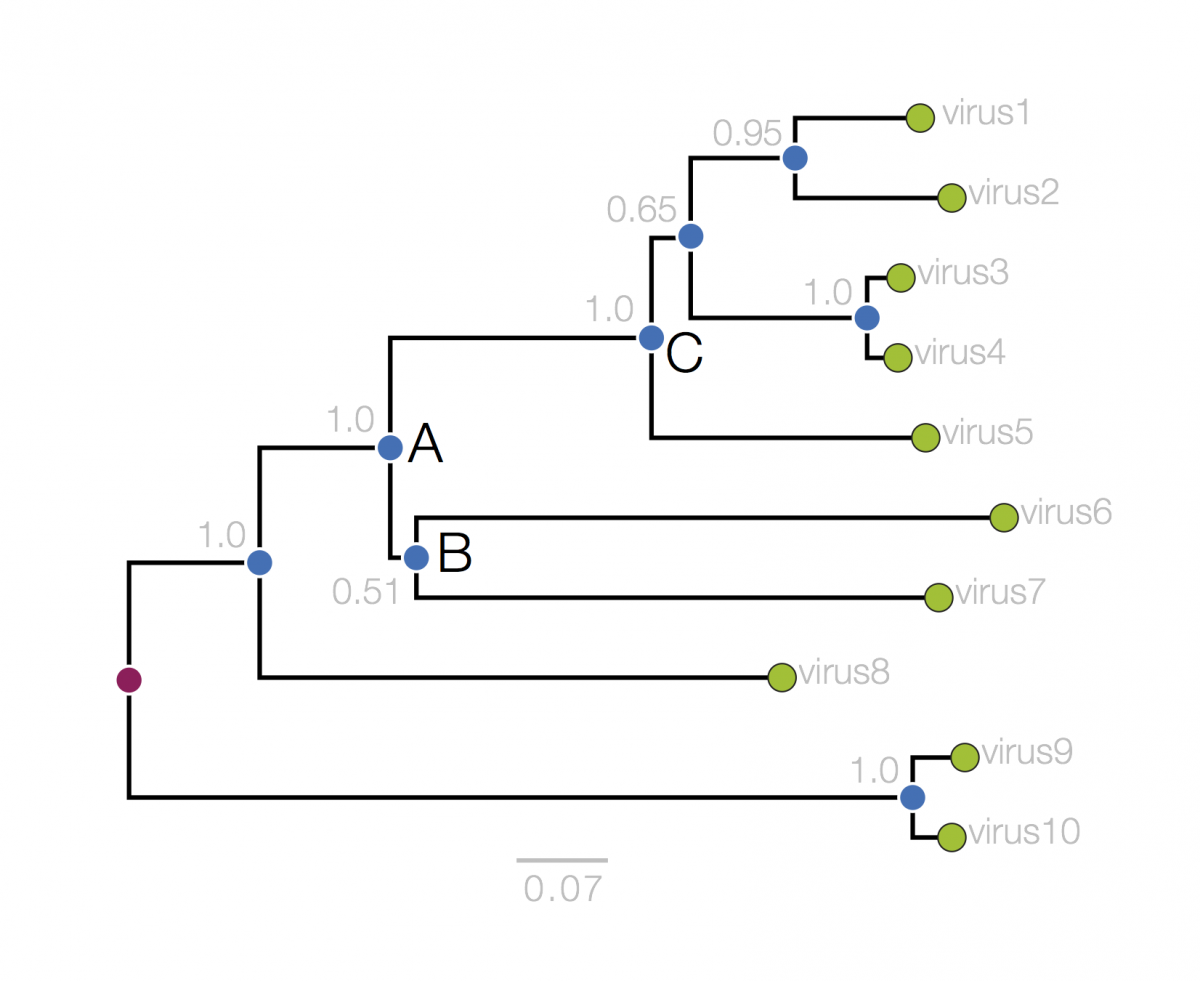
\includegraphics[width=0.6\textwidth]{phylogram_1a.png}
  \caption{An example of phylogenetic tree.}
  \label{fig:phytree}
\end{figure}

Phylogenetic trees are branching diagrams that show the evolutionary relationships between biological species. A weighted phylogenetic tree, with weights associated with its edges, captures the notion of genetic distances between species. By analyzing a weighted phygenetic tree, we understand not only \textit{how} but also \textit{how much} species are related to or different from one another. Figure \ref{fig:phytree} \footnote{Image taken from \url{http://epidemic.bio.ed.ac.uk/how_to_read_a_phylogeny}} features an artificial phylogentic tree of 10 viruses. Each virus is represented by a leave in the tree. Each internal node marks a milestone when a genetic divergence occurs. Notice that the lengths of the horizontal lines represents time periods. For instance, we can see that the divergence between virus 1 and virus 2 occurs before the divergence between virus 3 and virus 4. Phylogentic trees can be constructed from various distance metrics. In this example, the number assigned to each edge is the proportion of substitutions occuring on a sequence (the number of substituions divided by the length of the sequence). 

\subsection{Neighbor-joining algorithm}

We consider the problem of constructing a phylogentic tree from a set of protein sequences given their distance data. There are many approaches to tackle this problem. For instance, it can be framed as a hierarchical clustering problem, which has been extensively studied in the fields of data mining or machine learning and has efficient solution using statistical models. Although statistical approaches such as maximum likelihood methods have been employed to build these complex evolution trees, classical approaches such as the NJ algorithm has the advantage of being easy to implement and scalable to large datasets. 

Figure \ref{alg:nj} summarizes the NJ algorithm. The input for the NJ algorithm are a set $P$ of sequences (usually DNA or protein sequences) and a distance matrix $D$ where each entry is the distance between a pair of sequences. The NJ algorithm constructs the phylogentic tree from bottom up, going from leave to root. It starts with a forest of $N$ single-node trees, each of which represents a sequence. In each later step, the algorithm selects two trees in the forest, joins them into a single tree by connecting their roots to a newly formed root. This process repeats until there is only tree left in the forest.

In an intermediate step, the algorithm decides which two trees to join by computing a \textit{branch length} matrix based on the distance matrix. This matrix has $T \times T$ entries, where $T$ is the number of trees in the forest at the current step. Each entry of the matrix is computed as follows:  
\begin{equation}
  L_{i, j} = (T - 2) D_{i, j} - \sum_{k \in R}^n (D_{i, k} + D_{j, k})
  \label{eqn:branch}
\end{equation} where $R$ is the set of tree roots in the forest.

The NJ algorithm selects the pair ($x$, $y$) with the highest branching length and connects each of them to a new root, say $u$. The distances between the new root and the joined roots are:  
\begin{equation}
\begin{split}
& D_{u, x} = \frac{1}{2} D_{x, y} + \frac{1}{2(T - 2)} \left[ \sum_{k \in R} (D_{x, k} - D_{y, k}) \right] 
\\  
& D_{u, y} = D_{x, y} - D_{u, x}
\end{split}
\label{eqn:distance_joined}
\end{equation}

The distances between the new root and other roots are:
\begin{equation}
  D_{u, z} = \frac{1}{2} \left[ D_{x, z} + D_{y, z} - D_{x, y} \right], \ \ \ \text{for} \ z \neq x, y
\label{eqn:distance_nonjoined}
\end{equation}

\begin{figure}
  \begin{algorithmic}[1]
    \Function{Neighor-joining}{$P$, $D$}
      \State $R \leftarrow P$
      \For {$t = 1 \dots |P| - 2$}
        \State $T \leftarrow |R|$
        \For {$(i, j) \in R \times R$}
          \State Compute $L_{i, j}$ using equation \ref{eqn:branch} 
        \EndFor
        \State $(x, y) \leftarrow \arg \max L$
        \State Create new root $u$
        \State Compute distances from $u$ to other nodes using equations \ref{eqn:distance_joined} and \ref{eqn:distance_nonjoined}
        \State $R \leftarrow R \cup \{u\} \setminus \{x, y\}$
      \EndFor
    \EndFunction
  \end{algorithmic}
  \caption{\label{alg:nj}The neighbor-joining algorithm.}
\end{figure}

\subsection{Compute distances between sequences}

TODO: Ugur

\section{Experiment}
\subsection{Data}


\subsection{Results}
\subsubsection{Compare with other neighbor-joining implementations}

TODO: Khanh 

\subsubsection{Compare with other distance matrix implementations}

TODO: Ugur

\end{document}






